\chapter{Out-of-core Octree}
\label{chap:octree}

The term \textit{out of core} is used to describe the management of datasets whose size exceeds the available system memory. In this thesis, an out-of-core data structure is needed to handle large-scale point clouds efficiently. Section \ref{sec:octree_overview} gives an overview in the data structure that is used in this thesis, Section \ref{sec:octree_ooc} discusses the out-of-core organization of the octree. Section \ref{sec:octree_post} gives insight on the post-processing of the point cloud once the octree is created. Section \ref{sec:octree_culling} describes the task of creating a smaller representation of the octree that can be rendered efficiently. Section \ref{sec:octree_memory} concludes this chapter with a brief discussion about the memory consumption of this solution. 


\section{Overview}
\label{sec:octree_overview}

An octree is a hierarchical data structure in which each node represents a spatial region defined by a three-dimensional bounding box. If the decision is made to split a node, eight children are created, each representing an octant of the parent's bounding box. Due to the spatial subdivision properties, an octree is a popular data structure for storing point clouds. The spatial subdivision is a characteristic that is shared amongst almost all octree implementations. A characteristic that varies in each application is the composition of the content of octree's nodes. Various approaches exist that store point clouds in different ways. 

If an octree node is partitioned, the node's point set is distributed among the child nodes and the original node. 
Instant Points \cite{wimmer2006instant} keeps a small subset of points in the original node and distributes the remaining points according to the spatial position. This way, no points are duplicated, making it very memory efficient. 
Wand et al. \cite{wand2007interactive} distribute the entire point set among the node's children. The original node keeps an averaged subset of points. Thus, a multi-resolution representation of the point cloud is created at the cost of a larger memory footprint. 

This thesis uses an octree with a structure similar to that of Wand et al. If a node is partitioned, the point set is divided amongst its child nodes. A random subset of the original points is kept in the original node. Thus an efficient level-of-detail representation of the point cloud is created. 
The reason for not using the averaged subset is that the octree is tailored towards shape detection. This processing step is intended to be performed on original data. Moreover, for shape detection, each node is viewed as self-contained, such that no points from predecessor nodes are needed to represent the point cloud for this region and resolution entirely. This self-containment property is the reason why Wand et al.'s approach combined with the proposed subsampling technique is favored above an Instant-Points-like system. 

\par

Numerous decision rules exist that determine whether a node is split or not. A node is partitioned if the point count exceeds a threshold $n$. In this thesis, a decision based on the number of points in a node is favored as it keeps the number of points per node consistent.
Having a consistent number of points allows the variation in loading time and data size to be kept low. With nodes of consistent size, the runtime of procedures that are directly affected by the number of points for different nodes is similar as well. Therefore, such methods can be used in a context where immediate feedback is useful, such as user interactions, since the execution time can be estimated. In this thesis, a split threshold of 5000 points in a node is chosen. 


\section{Out-of-core Functionalities}
\label{sec:octree_ooc}
This thesis utilizes an out-of-core octree that stores each node's information and content separately. A \textit{chunk} describes a coherent portion of data that is stored in the cache file. Each octree node is built so that the node's information and node's content is stored in separate chunks. If an octree node is loaded into memory, the content of the node (i.e., the point set) remains on the hard drive. Only on explicit access, the point-set data is loaded into memory. Child nodes are stored as chunks as well. This interleaved structure of chunks allows for the minimal memory consumption for nodes, whose content is not needed directly. For example, bounding-box intersections can be calculated without the need of loading the point set into memory. Figure \ref{fig:out-of-core} shows the interleaved chunk structure of the out-of-core octree. Loading data into memory can only be done as long as free memory is available. Unused chunks of data are removed from memory after not being accessed for a distinct amount of time.

\begin{figure}
    \centering
    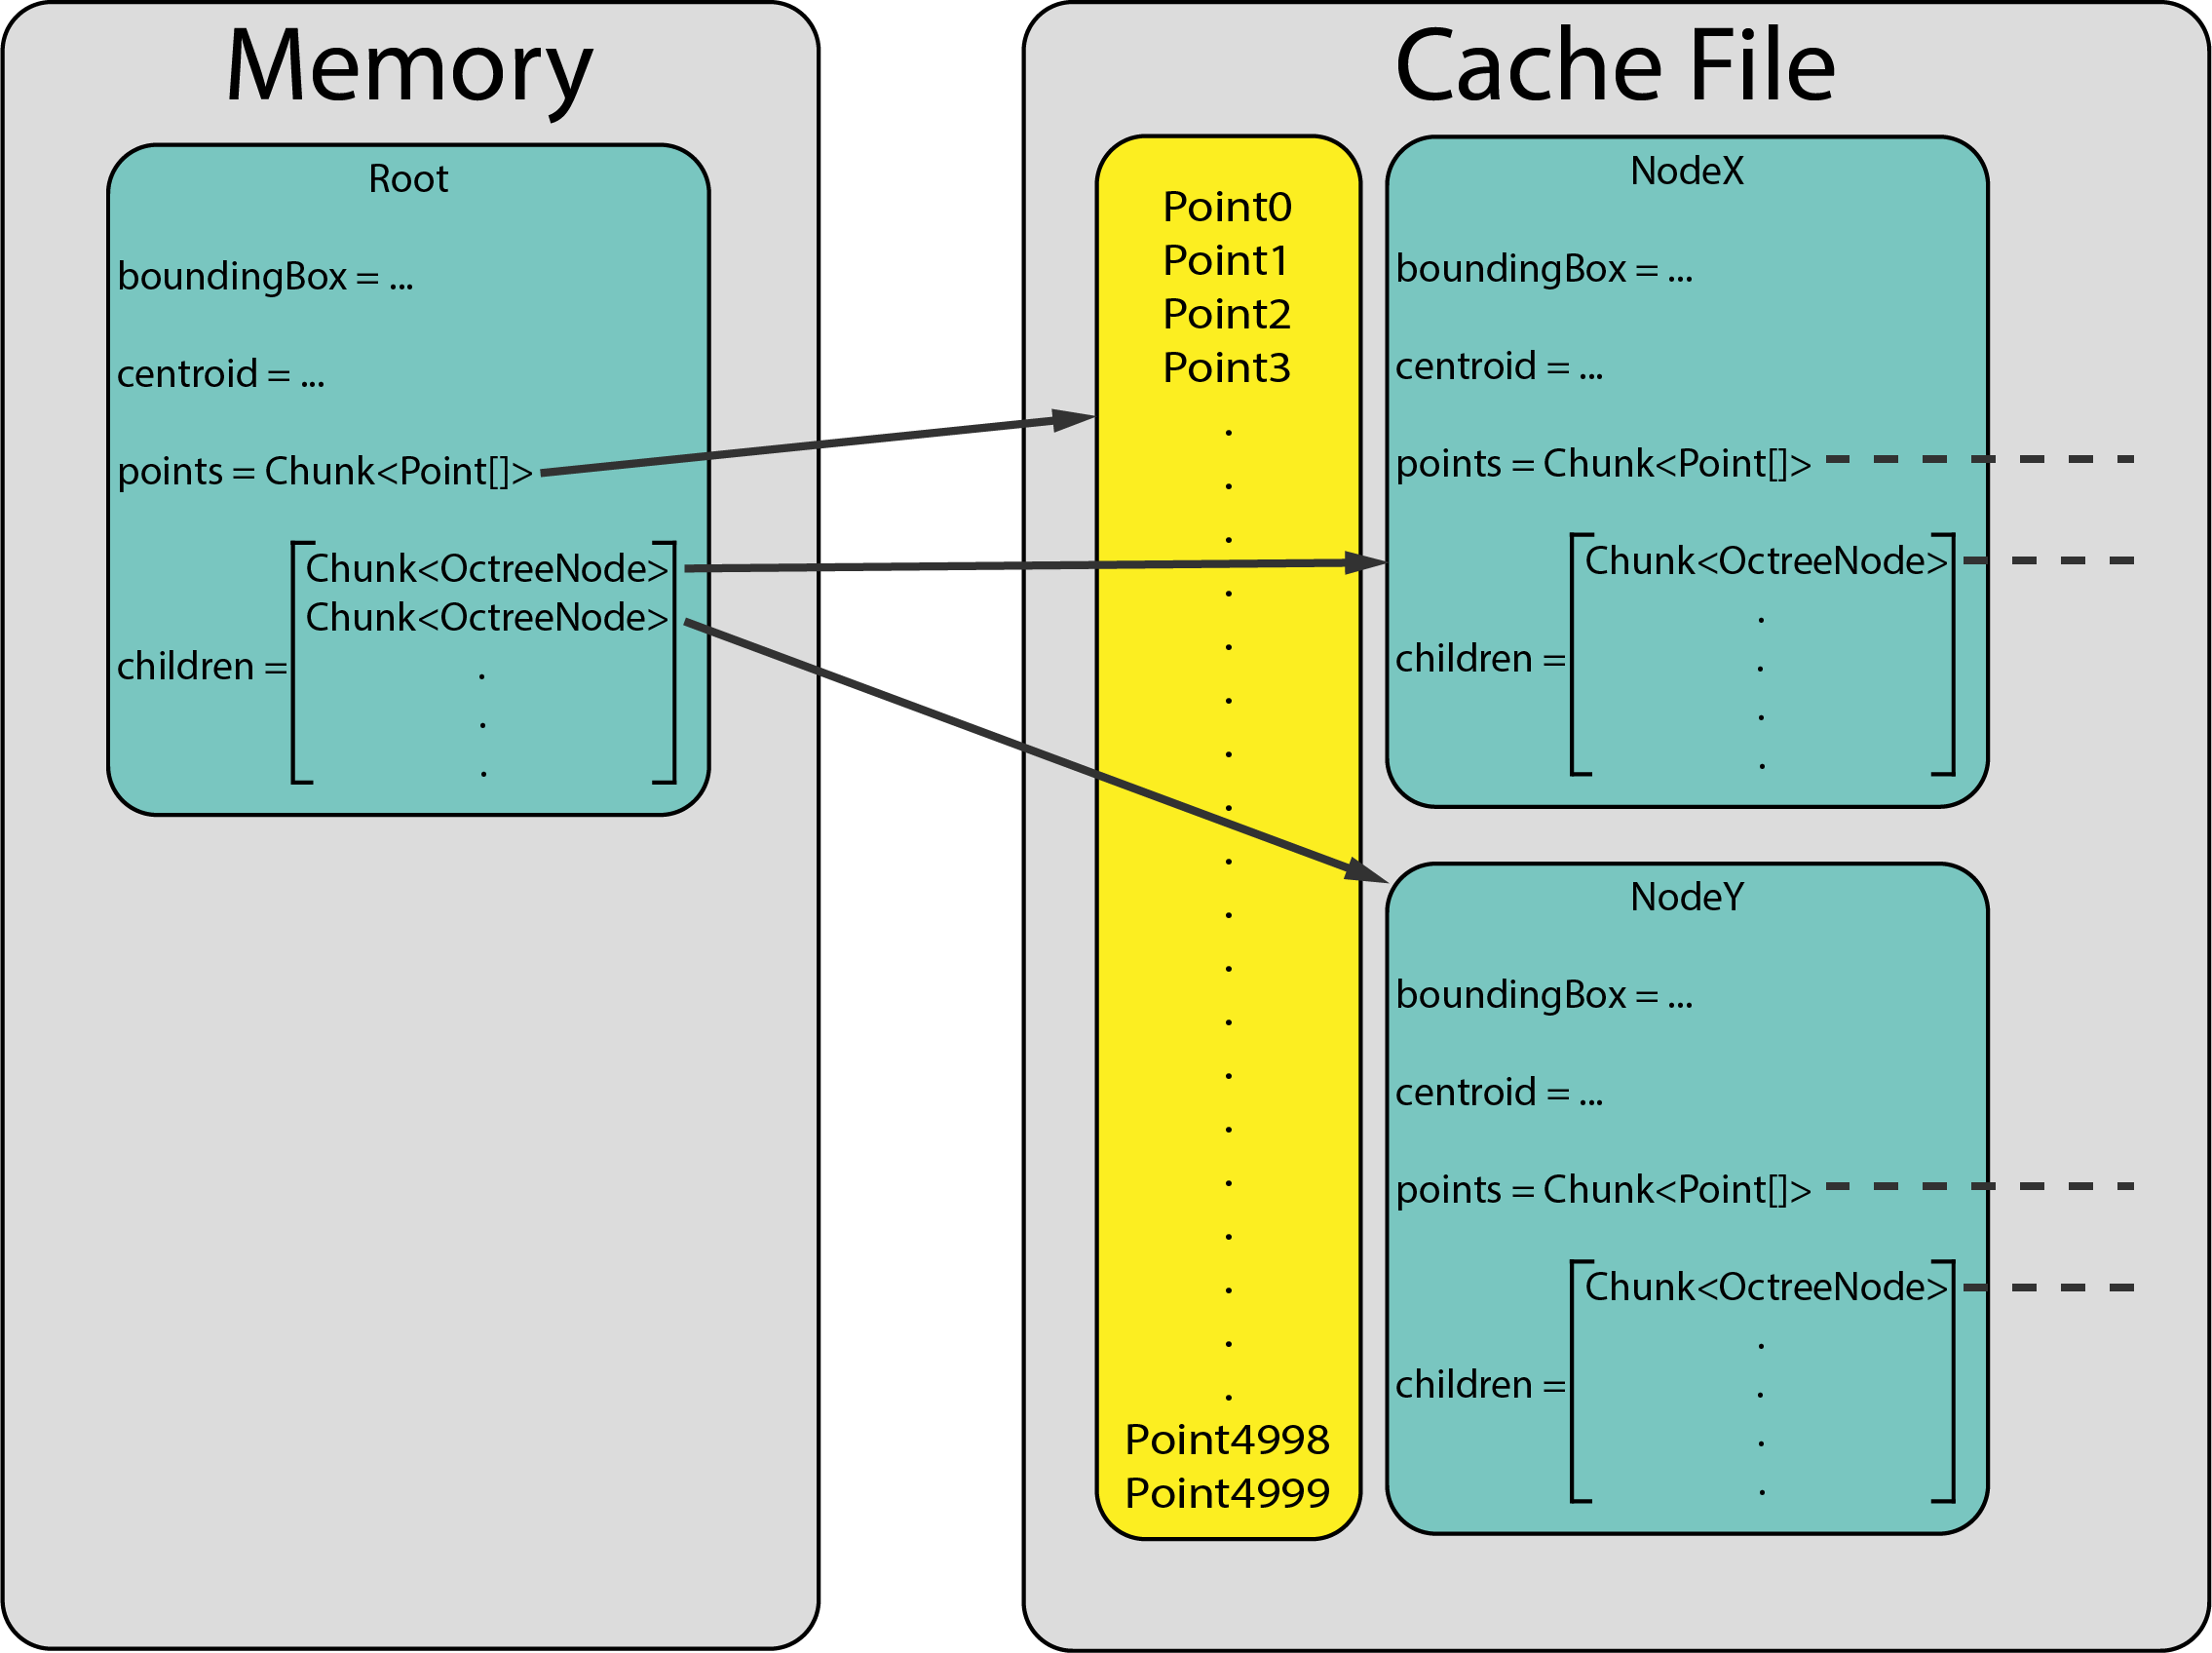
\includegraphics[width=0.5\textwidth]{Octree/out-of-core.png}
    \caption[Graphic describing the out-of-core structure of the octree]
        {This figure showcases the out-of-core structure of an octree with only the root node in the system memory(left). The point set remains in the cache file, as well as the node's children. Only necessary information, such as the node's bounding box and centroid are loaded into memory together with the node itself.}
    \label{fig:out-of-core}
\end{figure}


\section{Octree Postprocessing}
\label{sec:octree_post}
Point clouds often only contain information on position and color and lack distinct geometric features such as normal vectors. Normal vectors are significant for shape detection as they introduce information on the local curvature to the point cloud. After the octree build process is completed, additional properties are computed to enrich the dataset with more specific information. 


\subsection{rkd-Tree}

An rkd-tree \cite{tobler2011rkd} is an efficient data structure to perform fast n-nearest neighbor searches in static data sets. While the octree partitions the space into somewhat small regions, the rkd-tree further bisects the point set along the axes of the point space until only a single point is contained in each section. The rkd-tree improves the kd-tree by Friedman and Bentley \cite{friedman1975algorithm} by storing the radius of the sphere containing all points from the node's left and right subtrees. Thus, an early exclusion test with the sphere improves the performance of point queries. Instead of using a pointer-based binary search tree, the point array is rearranged so that the split point (i.e., median) for each bisection is located between the values of the one subtree and the values of the other subtree. Therefore, for each point in the array, only the index of the split dimension needs to be stored. 


\subsection{Normals}

For lighting and shape detection, each point must possess a normal vector. The local neighborhood determines a point's normal. Using the node's rkd-tree, a $k$-nearest-neighbor search is performed to retrieve the $k$ closest neighbors. Principal Component Analysis \cite{jolliffe2002principal} is used to fit a plane into the neighborhood. The plane's normal is defined by the eigenvector with the smallest eigenvalue. The plane's normal vector is used as the point's normal.


\subsection{Centroid}

The centroid of a node provides an indicator of the distribution of points in the octree node. The centroid is used as a target for the camera to focus on the presumably most dense part of the point cloud. 


\subsection{Density}

The density describes the average distance between a point and its nearest neighbor. The density increases with higher level-of-detail since more points are contained in a smaller region. To find the nearest neighbor, the node's rkd-tree is used again.


\section{Octree Culling}
\label{sec:octree_culling}

As a point cloud contains more data than the GPU can render in reasonable time, only points from those nodes are drawn that contribute to the currently viewed scene. The result of the culling operation is a new octree that contains only nodes that are currently rendered. The culled octree uses the same cached point information as the original octree. Thus, memory consumption is kept minimal. 

\par

A simple yet powerful culling heuristic is view-frustum culling. Nodes that are outside of the view frustum are discarded. By using view-frustum culling, whole branches of the octree are removed. The remaining branches are still too large to be rendered completely. A level-of-detail decision function determines whether or not a node should be rendered. Depending on the node's volume and distance to the near plane, a decision is made if the node should be rendered or not. 

\par

The heuristic culls hierarchically, meaning that if a parent is excluded, its children are as well. Thus, entire branches can be removed from the octree efficiently by only checking the parent node. If the octree is culled purely for rendering purposes, it is sufficient to collect the visible nodes in a set and use it for rendering. However, since interaction and processing tasks are performed on the viewed data, the hierarchical structure is kept intact. The intact hierarchy allows these tasks to exploit the octree structure and exclude entire branches of the culled octree with little computational cost. 


\section{Memory Consumption and Performance}
\label{sec:octree_memory}

The number of nodes from one level of detail to the next increases by the factor of $8$ (assuming that the octree is balanced and subdivided evenly). In reverse, when starting from the leaves, the number of nodes decreases by the factor of $\frac{1}{8}$. The upper bound of the relative size of the data stored in the entire octree is calculated from the geometric series: 


$$s = 1 + \frac{1}{8} + \frac{1}{64} + \frac{1}{512} + ... = \sum_{i = 0}^{\infty}{\frac{1}{8^i}} = \frac{8}{7}$$


To create the level-of-detail representation of the point cloud the size of the cache file and the number of stored points is increased by the factor of $\frac{8}{7}$. 

\par

All nodes from the culled octree are rendered, resulting in the multiple drawing of subsampled points from nodes with a lower level of detail. The previous calculations can be applied to estimate the overdraw when rendering the point cloud. The multiply drawn points account for $\sim$12\% of the entire point budget. The overdraw could be reduced by not drawing nodes, whose children are already drawn. However, the current implementation lacks this improvement. 
